\documentclass{standalone}
\usepackage{tikz}
\usetikzlibrary{shapes.multipart, arrows.meta}

\begin{document}
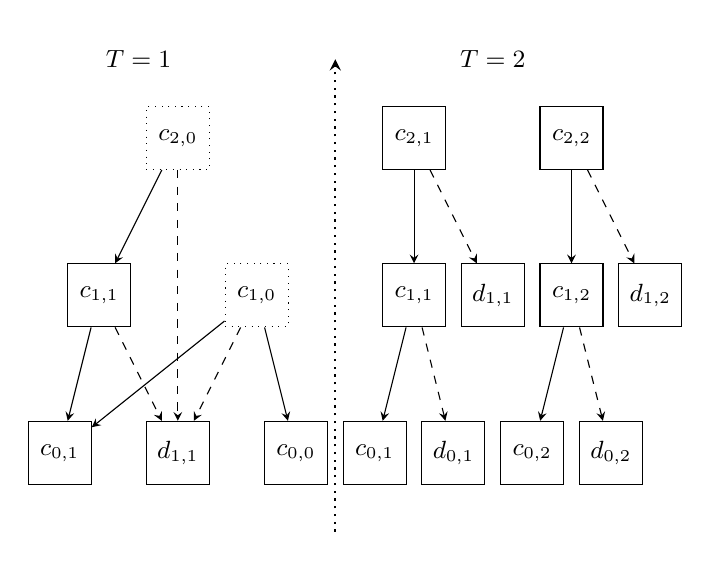
\begin{tikzpicture}[
  node distance=1.5cm and 2cm,
  every node/.style={rectangle, draw, minimum size=0.8cm, font=\small},
  every path/.style={-stealth},
  dotted path/.style={-stealth, dashed}
]

% Nodes for T=1
\node[draw, dotted] (c2_0_T1) at (0, 2) {$c_{2,0}$};
\node (c1_1_T1) at (-1, 0) {$c_{1,1}$};
\node[draw, dotted] (c1_0_T1) at (1, 0) {$c_{1,0}$};
\node (c0_1_T1) at (-1.5, -2) {$c_{0,1}$};
\node (d1_1_T1) at (0, -2) {$d_{1,1}$};
\node (c0_0_T1) at (1.5, -2) {$c_{0,0}$};

% Paths for T=1
\path (c2_0_T1) edge (c1_1_T1);
\path (c2_0_T1) edge[dotted path] (d1_1_T1);
\path (c1_1_T1) edge (c0_1_T1);
\path (c1_1_T1) edge[dotted path] (d1_1_T1);
\path (c1_0_T1) edge (c0_1_T1);
\path (c1_0_T1) edge[dotted path] (d1_1_T1);
\path (c1_0_T1) edge (c0_0_T1);

% Divider line
\draw[dotted, thick] (2, -3) -- (2, 3);

% Labels for T=1
\node[draw=none, fill=none] at (-0.5, 3) {$T=1$};

% Nodes for T=2
\node (c2_1_T2) at (3, 2) {$c_{2,1}$};
\node (c2_2_T2) at (5, 2) {$c_{2,2}$};
\node (c1_1_T2) at (3, 0) {$c_{1,1}$};
\node (c1_2_T2) at (5, 0) {$c_{1,2}$};
\node (d1_1_T2) at (4, 0) {$d_{1,1}$};
\node (d1_2_T2) at (6, 0) {$d_{1,2}$};
\node (c0_1_T2) at (2.5, -2) {$c_{0,1}$};
\node (d0_1_T2) at (3.5, -2) {$d_{0,1}$};
\node (c0_2_T2) at (4.5, -2) {$c_{0,2}$};
\node (d0_2_T2) at (5.5, -2) {$d_{0,2}$};

% Paths for T=2
\path (c2_1_T2) edge (c1_1_T2);
\path (c2_1_T2) edge[dotted path] (d1_1_T2);
\path (c2_2_T2) edge (c1_2_T2);
\path (c2_2_T2) edge[dotted path] (d1_2_T2);
\path (c1_1_T2) edge (c0_1_T2);
\path (c1_1_T2) edge[dotted path] (d0_1_T2);
\path (c1_2_T2) edge (c0_2_T2);
\path (c1_2_T2) edge[dotted path] (d0_2_T2);

% Labels for T=2
\node[draw=none, fill=none] at (4, 3) {$T=2$};

\end{tikzpicture}
\end{document}